\chapter{Materials and Methods}\label{ch:materials_methods}

This chapter outlines the methodological foundation that supports the design, execution, and analysis of the research found in this manuscript. Its purpose is to establish how the research questions introduced in Section~\ref{sec:research_questions_objectives} are translated into an empirical workflow that spans dataset construction, model inferencing, and model assessment via statistical analysis.

Section~\ref{sec:research_framework} introduces the research framework. It describes the conceptual structure of the six-phase pipeline, explains how artifacts produced at each stage feed forward into subsequent phases, and shows how this architecture aligns to the contributions, effectively bridging the gap between the research objectives and the empirical procedures implemented in the remainder of the chapter.

Section \ref{sec:infrastructure} details the computational and software infrastructure required to perform the research. It covers hardware and software requirements required to have reproducible experimentation, as well as external services leveraged that provide dataset hosting and model access.

Section \ref{sec:dataset_construction} describes the workflow transforming the SysEngBench dataset. It covers the generation of position-rotated variants, and the pipeline used to convert questions from \acp{mcq} to \acp{osq}.

Section \ref{sec:evaluation_procedures} explains how the datasets are used to evaluate language models. It documents the task configurations of evaluation harness for all question formats. It also describes the LLM-as-a-Judge process used to evaluate \acp{osq}.

Section \ref{sec:analytical_approach} outlines the statistical techniques used to interpret the results. It introduces the three analytic pillars — position bias analysis, format comparison between \ac{mcq} and \ac{osq} modalities, and token-cost efficiency. 




\section{Methodological Framing and Traceability to Research Objectives}
\label{sec:ch3_framing}

Chapter~\ref{ch:introduction} defined a set of Research Objectives in Section \ref{sec:research_objectives} that constitute the intentional, completable actions required to answer the research questions in Section \ref{sec:research_questions}. This research was executed through an empirical pipeline that is organized primarily around the Research Objectives to preserve traceability between declared intent and implemented methodology.

The pipeline describes the chronological sequencing of work (e.g., dataset derivation, inference execution, scoring, and analysis). However, chronological sequencing alone does not make explicit how each step contributes to the production of qualification-relevant evidence. Because this dissertation frames model evaluation as a qualification problem that requires modality-aware, robustness-aware, and cost-aware evidence, Chapter~\ref{ch:materials_methods} is structured around the objectives themselves. Each objective defines the work performed, the artifacts produced, and the evidence generated. 

The only objective not included in this chapter is Objective 7, which is met with Chapter 5 (synthesis).

The execution environment and reproducibility controls that underlie all objectives are described first. Subsequent sections correspond directly to the Research Objectives listed in Section~\ref{sec:research_objectives}. 




\subsection{Pipeline as Execution Backbone}
\label{subsec:ch3_pipeline_backbone}

This section presents the overall methodological framework that connects the research questions posed in Chapter~\ref{ch:introduction} to the data collection, evaluation, and analysis procedures described in subsequent sections. The framework follows a pipeline that transforms the base SysEngBench \cite{bell_rabellsysengbench_2024} dataset through multiple processing stages, evaluates \acp{llm} across both \ac{mcq} and \ac{osq} question formats, and performs comprehensive statistical analysis of the results.

Figure \ref{fig:modality_eval_pipeline} presents the high-level data flow through the pipeline. Each step produces well-defined artifacts, including datasets, model responses, judging scores, or analysis outputs that serve as inputs to subsequent steps. 

\begin{figure}[htbp]
    \centering
    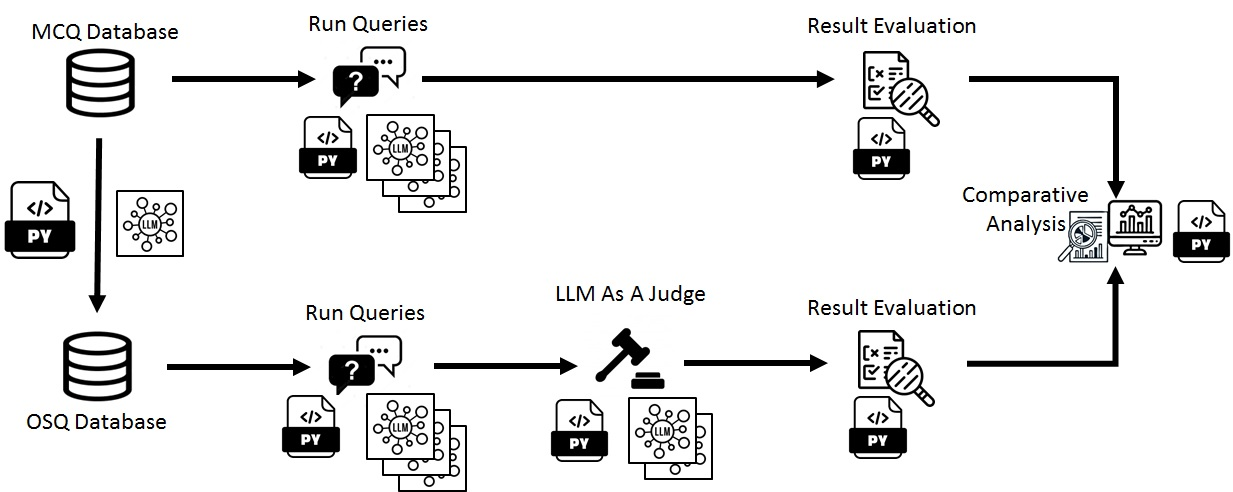
\includegraphics[width=0.9\textwidth]{figs/ch3/3.1/modality-evaluation-pipeline.jpg}
    \caption{Modality Evaluation Pipeline}
    \label{fig:modality_eval_pipeline}
\end{figure}


% ---------------------------------------------------------
\section{Execution Environment and Reproducibility Controls}
\label{sec:ch3_infrastructure}

This section details the software stack and computational infrastructure used throughout the research pipeline. It functions as the shared substrate for all objectives: dataset derivation, standardized inference, OSQ scoring via LLM-as-a-judge, and token/cost accounting were performed within a controlled and logged environment to support traceability and reproducibility.

\subsection{Software Stack}\label{subsec:ch3_software_stack}

The complete software stack is summarized in Table \ref{tab:software_stack}. The full list python packages used are included in the `requirements.txt` in the dissertation repository hosted on GitHub at \texttt{ryan-a-bell/dissertation}.

\begin{table}[h!]
    \centering
    \caption{{Software Stack Components and Their Roles in the Research Pipeline}}
    \label{tab:software_stack}
    \rowcolors{0}{}{} % Turn off row colors
    \resizebox{\columnwidth}{!}{%
    \begin{tabular}{ccc}
    \hline
    \textbf{Component} & \textbf{Version} & \textbf{Purpose} \\
    \hline
    Python & 3.11+ & Primary programming language. \\
    Pandas & 2.1+ & Data manipulation and CSV processing. \\
    NumPy & 1.24+ & Numerical computations. \\
    SciPy & 1.11+ & Statistical testing. \\
    scikit-learn & 1.3+ & Machine learning utilities. \\
    Matplotlib & 3.8+ & Visualization. \\
    Seaborn & 0.13+ & Statistical graphics. \\
    datasets & 2.14+ & HuggingFace dataset loading. \\
    lm-evaluation-harness & 0.4+ & Standardized LLM evaluation. \\
    Ollama & 0.13.0+ & Local LLM serving. \\
    openai & 1.x & API client for judge models. \\
    tqdm & 4.66+ & Progress tracking. \\
    \hline
    \end{tabular}%
    }
\end{table}


\subsection{Compute Environment}
\label{subsec:ch3_compute_environment}

%%% ADD GPUaaS somewhere


Model inference required GPU resources due to the large number of models evaluated and the size of some models that were over 272B parameters. GPU compute was provisioned through RunPod\footnote{\url{https://www.runpod.io/}}, a cloud GPU platform offering on-demand access to NVIDIA A40, A100, H200 SXM, among other \acp{gpu}. This enabled rapid iteration on evaluation configurations, consistent environment setup, and the ability to evaluate large models that were impractical to host locally.

GPU selection was driven primarily by each model’s memory requirements. Larger models were placed on the highest-capacity, highest-performance GPUs available, ensuring sufficient VRAM headroom for inference overhead and optimized execution. Smaller models were scheduled onto appropriately sized GPU instances to maintain efficient resource utilization.





Each RunPod instance was configured with:
\begin{itemize}
    \item PyTorch container template (CUDA 12.1, PyTorch 2.1+)
    \item Exposed port 11434 for Ollama API access
    \item Persistent volume storage for model weights
    \item SSH access for command-line operations
    \item JupyterLab interface for interactive notebook for debugging
\end{itemize}

 Ollama\footnote{\url{https://ollama.ai/}} served as the \ac{llm} inferencing service, providing an OpenAI-compatible API endpoint at \texttt{http://localhost:11434/v1/chat/completions}. Ollama handles model loading, memory management, and efficient batched inference. Models were pulled systematically from the Ollama registry using \texttt{ollama pull <model\_name>} and verified with \texttt{ollama list}.

Primary development occurred on a local workstation running Windows 11 with Python 3.12.4. Jupyter notebooks were used for exploratory analysis and prototyping, while production evaluation scripts were executed on RunPod GPU instances. 

The Figure \ref{fig:icd-scalable-workers} illustrates a scalable GPU-based inference and computation workflow built on top of RunPod, although the framework is GPU provider agnostic. At the top, a user interacts through a Jupyter Notebook running in a local execution environment. This environment spawns multiple subprocesses — each acting as a “RunPod Runner” — which communicate with remote GPU pods. These subprocesses form the client-side layer that initiates tasks, sends workloads to the cloud, and receives results. Their interaction with the notebook is bidirectional, enabling parallel job submission and coordination from a single interactive workspace.

Beneath the local layer is the RunPod cloud infrastructure, which hosts an orchestrator and a pool of GPU-backed pods. The orchestrator manages communication channels, routing tasks from local subprocesses to the appropriate pods via dedicated DirectChannel links. Each pod contains a GPU Runner responsible for executing the assigned workload. The architecture supports multiple pods (1 through N), enabling horizontal scaling as demand grows.

\begin{figure}[htbp]
    \centering
    
\includegraphics[width=0.9\textwidth]{figs/ch3/3.2/icd-runpod-workers.png}
    \caption{Architectural Interconnect for Scalable Workers}
    \label{fig:icd-scalable-workers}
\end{figure}

To reduce sources of uncontrolled variance, inference was performed with deterministic decoding settings where supported (see Section~\ref{subsec:ch3_determinism}). In addition, model and infrastructure heterogeneity (local inference vs. hosted APIs) was treated as an explicit experimental reality rather than hidden complexity; the workflow retains sufficient run metadata to reconstruct which provider, model identifier, and configuration produced each output.




\subsection{External Services and APIs}

Two external services were used to support this research:

\paragraph{HuggingFace} The SysEngBench dataset is hosted on HuggingFace Hub at \texttt{rabell/SysEngBench} \cite{bell_rabellsysengbench_2024} and accessed via the \texttt{datasets} library with an authentication token. The other variants of SysEngBench, including the MCQ variants SysEngBench-A, SysEngBench-B, SysEngBench-C, SysEngBench-D, as well as converted OSQ dataset SysEngBench-OSQ may be found on HuggingFace for reproducibility.

\paragraph{OpenRouter} OpenRouter\footnote{\url{https://openrouter.ai/}} provided unified API access to proprietary models (e.g. GPT-5, Claude, Gemini) and larger open-source models not suitable for local execution. This service enabled easy model switching via a single API endpoint while maintaining usage tracking and cost monitoring. All API calls use temperature as 0.0 for deterministic outputs.

\begin{itemize}
    \item \textbf{Hugging Face} was used to retrieve and version benchmark artifacts (datasets), enabling stable dataset identifiers and reproducible access patterns.
    \item \textbf{OpenRouter} was used to access proprietary foundation models through a single API endpoint. This simplified evaluation orchestration across multiple providers while preserving consistent logging and configuration capture.
\end{itemize}

OpenRouter exposes a common parameter interface (e.g., temperature) and routes requests to provider endpoints. Temperature was set to \texttt{0.0} to remove output variance across repeated runs. Parameter defaults and supported options vary across providers, so model-specific capability constraints were handled explicitly in the run configuration rather than assumed.\footnote{\url{https://openrouter.ai/docs/api/reference/parameters}}



\subsection{Evaluation Harness and Tooling}
\label{subsec:ch3_harness}

% tools to employ -- include tools like vllm, ollama, lm studio, llama.cpp etc

Model evaluation was implemented using the Language Model Evaluation Harness (\texttt{lm-eval}), an open-source framework that standardizes task definitions, prompt formatting, inference orchestration, and result aggregation across model backends.\footnote{\url{https://github.com/EleutherAI/lm-evaluation-harness}} The harness provides a consistent interface for evaluating both local models and API-accessed models, supporting reproducible comparisons across heterogeneous systems.

% Recommended citation (add to BibTeX):
% - Biderman et al. "lm-evaluation-harness" (arXiv:2405.14782) for a citable reference to lm-eval.

For local inference, models were hosted using \texttt{Ollama} where applicable, enabling consistent invocation across multiple open-weight model families. For API-accessed models, requests were issued through a unified gateway (Section~\ref{subsec:ch3_external_services}) to standardize request formatting and logging. Auxiliary scripts were used for dataset processing, rubric generation, and post-hoc analysis. All tooling was integrated within a repository-managed workflow to ensure that dataset versions, prompts, and evaluation configurations remain synchronized with the reported results.


All MCQ and OSQ evaluations, as well as the judge scoring evaluations used lm-evaluation-harness \cite{eleutherai_eleutherailm-evaluation-harness_2024}, a standardized framework for \ac{llm} benchmarking. This framework provides:
\begin{itemize}
    \item Consistent prompt formatting across models
    \item Automatic metric calculation (accuracy, per-category accuracy)
    \item Structured output (JSON results, JSONL sample logs)
    \item Support for custom tasks via YAML configuration
\end{itemize}



\subsection{Dataset Hosting, Versioning, and Artifact Management}
\label{subsec:ch3_dataset_versioning}

SysEngBench and all derived datasets were managed as versioned artifacts to support traceability between dataset construction and evaluation outcomes. The base dataset was retrieved from Hugging Face (\texttt{rabell/SysEngBench}) via API access. Derived datasets (OSQ-converted sets and MCQ positional variants) were constructed deterministically from the base dataset and stored with explicit version identifiers (e.g. -A, -B, -C, -D, -OSQ).

Versioning discipline is essential for traceability, even minor modifications to prompt templates, item filtering criteria, or answer-option rotation rules can affect measured performance. Accordingly, dataset derivation scripts were tracked under version control, and dataset releases were associated with immutable references (e.g., commit hashes and dataset tags) in the dissertation repository.

% Recommended citation (add to BibTeX) for dataset tooling:
% - Lhoest et al. 2021, "Datasets: A Community Library for Natural Language Processing" (EMNLP demo / arXiv:2109.02846)

\paragraph{Version Control and Tracking} All code, notebooks, and analysis scripts were version-controlled using Git and hosted on GitHub at \texttt{ryan-a-bell/dissertation}. 

\subsection{Data Management and Reproducibility}

To ensure reproducibility:
\begin{itemize}
    \item All datasets are versioned and publicly accessible on HuggingFace \cite{bell_rabellsysengbench_2024}
    \item Model inference used temperature=0.0 for deterministic generation
    \item Complete evaluation logs with timestamps were retained
    \item Environment specifications captured in \texttt{requirements.txt}
    \item All code and notebooks publicly available in the GitHub repository at \texttt{ryan-a-bell/dissertation}
\end{itemize}

Sensitive credentials such as personal HuggingFace tokens or OpenRouter API keys were stored in a \texttt{.env} file excluded from version control, but a template for use has been provided in \texttt{.env.template}.


\subsection{Determinism Controls and Run Standardization}
\label{subsec:ch3_determinism}

Across all inference runs, settings were standardized to reduce avoidable variance and improve comparability:

\begin{itemize}
    \item \textbf{Decoding determinism:} temperature set to 0.0, with consistent max token limits and stop sequences.
    \item \textbf{Prompt standardization:} task templates and instruction framing were held fixed within each evaluation condition.
    \item \textbf{Retry policy:} transient API failures or invalid outputs were retried under a controlled policy, and failures were logged as artifacts. 
    \item %%% retry policy -- it was re-ran. the process is idempotent so results w/o the transient api failures etc were removed when replaced with the correct results.
\end{itemize}

These controls support the dissertation’s framing of evaluation as qualification evidence: uncontrolled procedural variance weakens the interpretability of observed differences and can produce misleading deltas across models and modalities.


\subsection{Logging, Artifact Retention, and Auditability}
\label{subsec:ch3_logging}
To support repeatability and retrospective auditing, the following artifacts were retained:

\begin{itemize}
    \item \textbf{Dataset artifacts:} dataset versions, item identifiers, conversion outputs, and rotation maps.
    \item \textbf{Inference artifacts:} prompts, raw model responses, response metadata (model id, backend/provider, decoding parameters).
    \item \textbf{Scoring artifacts:} judge prompts, judge outputs, structured rubric scores, and stability check outputs (where applicable).
    \item \textbf{Analysis artifacts:} aggregated result tables and statistical test outputs used to generate reported figures and claims.
\end{itemize}

This design enables downstream validation and supports the claim that results can be reproduced given the same model versions and evaluation configurations.


\subsection{Token Accounting and Cost Instrumentation}
\label{subsec:ch3_token_tracking}

Token usage and response length were measured as first-class quantities for Objective 6. For each inference call, input and output token counts were recorded when supported by the backend. For API-accessed models, provider usage fields were captured when available; for local inference, token counts were computed using the model’s tokenizer or proxy estimation procedures consistent across the evaluated set.
%%% USED LM-EVAL'S LIMIT FOR TOKENS. ADD THAT CITATION HERE.

The total cost of OSQ evaluation includes both \emph{generation cost} (model answering) and \emph{scoring cost} (judge inference). This “two-pass” structure is central to cost-aware qualification reasoning: OSQ evaluation is not only higher-variance in output form, but also higher-cost due to rubric-based scoring overhead.
%% REWORD ABOVE. LIKELY TO REMOVE MOST BUT KEEP THAT WE CAN COMPUTE THE SCORING COST TOO (FOCUSED ON GENERATION COST, NOT THE CSOT OF JUDGING)
















% ---------------------------------------------------------
\section{Objective 1: Benchmark Curation and Derivative Construction}
\label{sec:ch3_obj1}

\subsection{Baseline Benchmark Acquisition and Characteristics}
\label{subsec:ch3_obj1_baseline}

SysEngBench is a \ac{mcq} benchmark for systems engineering, aligned to the INCOSE Systems Engineering Handbook \cite{bell_IntroducingSysEngBenchNovel_2024}. The dataset was downloaded from Hugging Face (\texttt{rabell/SysEngBench}) via API access \cite{bell_RabellSysEngBenchDatasets_2024}. The test split contains 1,144 questions spanning six major \ac{incose} knowledge areas and 20 sub-categories.

Each question record includes the following fields:
\begin{itemize}
    \item \texttt{question\_id}: Unique numeric identifier.
    \item \texttt{question}: Question stem text.
    \item \texttt{choices}: Four answer choices (A--D).
    \item \texttt{answer}: Correct answer (A--D).
    \item \texttt{justification}: A short rationale supporting the correct answer.
    \item \texttt{category}: INCOSE knowledge area category label.
    \item \texttt{subcategory}: INCOSE subcategory label.
\end{itemize}

These fields provide the minimum metadata required to support both robustness analysis in the MCQ setting and conversion to OSQ variants with canonical expected answers and rubrics (Objective 2).

An extensive analysis of the benchmark was conducted in \cite{Bell2025SysEngBench}, still under review with Wiley that includes sub-categories with distributions visualized using bar charts, pie charts, and stacked visualizations to express the coverage of the benchmark across the systems engineering domain.


\subsection{Construction of MCQ Robustness Variants}
\label{subsec:ch3_obj1_mcq_variants}

To detect position bias in model responses to \acp{mcq}, as demonstrated in \cite{zheng_large_2024}, four variants of the SysEngBench dataset were generated with correct answers systematically rotated to positions A, B, C, and D. This approach enables statistical testing for underlying preference for answer positions.

The rotation procedure preserves question content and choice semantics while permuting answer-option ordering. For each base item, a rotation map is computed such that each of the four variants places the correct answer in a different position while maintaining a consistent permutation structure over the four options. This produces four aligned datasets:

\begin{itemize}
    \item \textbf{SysEngBench-A\footnote{\url{https://huggingface.co/datasets/rabell/SysEngBench-A}}}: Correct answer at position A (label=0)
    \item \textbf{SysEngBench-B\footnote{\url{https://huggingface.co/datasets/rabell/SysEngBench-B}}}: Correct answer at position B (label=1)
    \item \textbf{SysEngBench-C\footnote{\url{https://huggingface.co/datasets/rabell/SysEngBench-C}}}: Correct answer at position C (label=2)
    \item \textbf{SysEngBench-D\footnote{\url{https://huggingface.co/datasets/rabell/SysEngBench-D}}}: Correct answer at position D (label=3)
\end{itemize}

Because each variant contains the same questions under systematic reordering, differences in accuracy across variants can be attributed to positional sensitivity rather than content differences.

Figure~\ref{fig:phase3_rotation} illustrates the rotation process.

\begin{figure}[htbp]
    \centering
    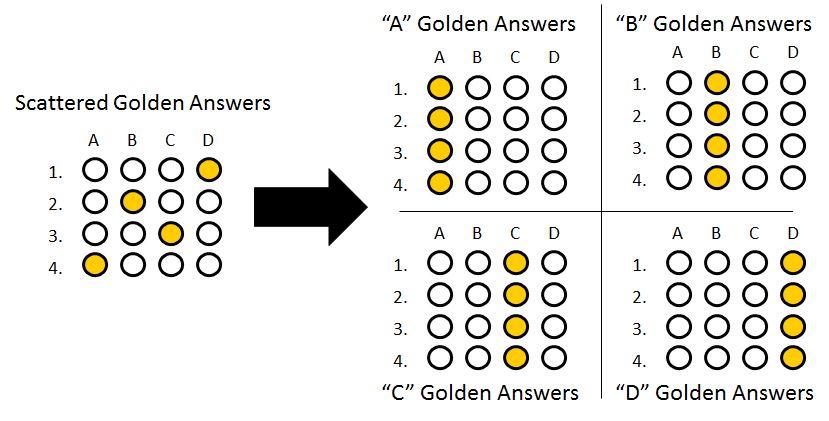
\includegraphics[width=0.9\textwidth]{figs/ch3/mcq-distractor-datasets.png}
    \caption{MCQ Position Variant Generation}
    \label{fig:phase3_rotation}
\end{figure}



\subsection{MCQ to OSQ Conversion Process}
\label{subsec:ch3_obj1_alignment}

The conversion process from \ac{mcq} to \ac{osq} consists of two sequential stages: (1) suitability classification, and (2) conversion with rubric generation. Figure \ref{fig:mcq-to-osq} illustrates the complete pipeline.


\begin{figure}[htbp]
    \centering

    \subfloat[MCQ Check for Convert-ability]{%
        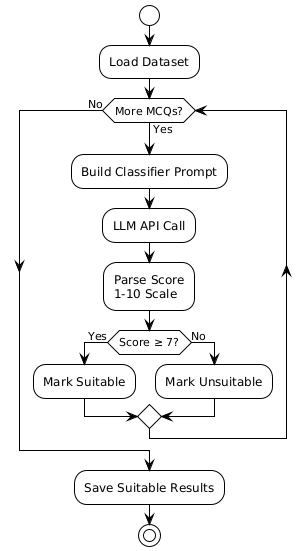
\includegraphics[width=0.48\textwidth]{figs/ch3/3.3/filter-mcqs.png}
    }\hfill
    \subfloat[Conversion of MCQ to OSQ]{%
        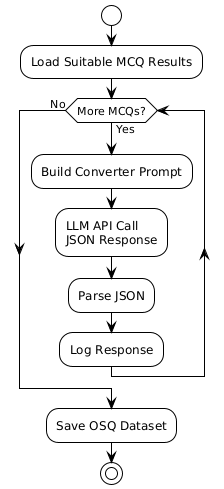
\includegraphics[width=0.48\textwidth]{figs/ch3/3.3/convert-mcq-to-osq.png}
    }

    \caption{Multiple Choice Question to Open Style Question Workflow}
    \label{fig:mcq-to-osq}
\end{figure}

Stage 1 classifies each MCQ for OSQ suitability across five key elements. Questions scoring $\geq 7/10$ proceed to Stage 2, where conversion generates a OSQ prompt, expected answer, grading rubric, and Bloom's taxonomy classification. 

\paragraph{Stage 1: Suitability Classification}

The suitability classifier filters out items where the OSQ form would be ambiguous, underspecified, or would fail to preserve the original measurement intent. Suitable items are then converted into OSQs and paired with canonical expected answers and structured rubrics.
%% COMBINE THESE TWO PARAGRAPHS
Not all multiple-choice questions are suitable for conversion to open-ended format. Questions requiring visual diagrams, those with highly ambiguous correct answers, or those where the distractor options provide essential context may not translate well.

Each of the \acp{mcq} was evaluated by ChatGPT-5 via OpenRouter with a temperature of 0 across five key elements, including:

\begin{enumerate}
    \item \textbf{Assessability}: Can the answer be evaluated objectively in open-ended format?
    \item \textbf{Canonical Answer Clarity}: Is there a well-defined expected answer?
    \item \textbf{Ambiguity}: Is the question clear without the MCQ structure?
    \item \textbf{Scope Appropriateness}: Is the expected answer reasonable in length for short-answer format?
    \item \textbf{Intent Preservation}: Can the original knowledge construct be maintained without MCQ options?
\end{enumerate}

The \ac{llm} returned a structured JSON response containing:
\begin{lstlisting}[language=json,
    basicstyle=\ttfamily\footnotesize,
    caption={Structure of the LLM evaluation output},
    label={lst:llm-json}
]

{
  "suitability_score": <1-10>,
  "justification": "<reasoning>",
  "dimension_scores": {
    "assessability": <1-10>,
    "canonical_answer": <1-10>,
    "ambiguity": <1-10>,
    "scope": <1-10>,
    "intent_preservation": <1-10>
  }
}
\end{lstlisting}

The complete classification prompt is provided in Appendix~\ref{appendix-a}.

\paragraph{Stage 2: Conversion with Rubric Generation}

For each suitable \ac{mcq}, ChatGPT-5 was used to perform the conversion. The conversion process:

\begin{itemize}
    \item Removed MCQ-specific artifacts (e.g., ``which of the following'', explicit A/B/C/D options)
    \item Maintained the original intent (e.g., definition recall remains recall, not application)
    \item Preserved any numerical calculations or technical specifications
    \item Generated a canonical expected answer based on the original correct choice
    \item Created a grading rubric with three levels:
    \begin{itemize}
        \item \textbf{Full credit}: Criteria for complete correct answer
        \item \textbf{Partial credit}: Criteria for partially correct answer
        \item \textbf{No credit}: Conditions warranting no credit
    \end{itemize}
    \item Assigned Bloom's taxonomy level (Remember, Understand, Apply, Analyze, Evaluate, Create)
\end{itemize}

The conversion prompt explicitly instructed the LLM to ``keep the construct and difficulty comparable'' for \acp{osq}, maintaining parity with the original \ac{mcq} construct.

The response for the conversion prompt is a structured JSON:

\begin{lstlisting}[language=json,
    basicstyle=\ttfamily\footnotesize,
    caption={Structure of the OSQ generation prompt},
    label={lst:osq-json}
]
{
  "osq_prompt": "<open-ended question>",
  "expected_answer": "<canonical answer>",
  "rubric": {
    "full_credit": "<criteria>",
    "partial_credit": "<criteria>",
    "no_credit": "<criteria>"
  },
  "blooms_level": "<taxonomy level>",
  "blooms_justification": "<reasoning>"
}
\end{lstlisting}

A sample question from a successful conversion process MCQ to OSQ example is provided in Table~\ref{tab:conversion_example}.

\begin{table}[h!]
    \centering
    \caption{{Example MCQ to OSQ Conversion Showing Original Question, OSQ Converted Question, and Grading Rubric}}
    \label{tab:conversion_example}
    \rowcolors{0}{}{} % Turn off row colors
    \resizebox{\columnwidth}{!}{%
    \begin{tabular}{ccp{0.7\textwidth}}
    \hline
    \textbf{Field} & \textbf{Content} & \\
    \hline

    \textbf{Original MCQ} &
    \multicolumn{2}{p{0.7\textwidth}}{%
        \begin{minipage}[t]{\linewidth}
        What is the primary purpose of stakeholder analysis in systems engineering?
        \begin{itemize}[noitemsep,topsep=0pt]
            \item[A.] To identify project funding sources
            \item[B.] To understand stakeholder needs and concerns
            \item[C.] To assign project responsibilities
            \item[D.] To develop marketing strategies
        \end{itemize}
        \textbf{Answer}: B
        \end{minipage}
    } \\
    \addlinespace[0.7em]

    \textbf{OSQ Prompt} &
    \multicolumn{2}{p{0.7\textwidth}}{%
        What is the primary purpose of stakeholder analysis in systems engineering?
    } \\
    \addlinespace[0.7em]

    \textbf{Expected Answer} &
    \multicolumn{2}{p{0.7\textwidth}}{%
        To understand stakeholder needs and concerns.
    } \\
    \addlinespace[0.7em]

    \textbf{Full Credit} &
    \multicolumn{2}{p{0.7\textwidth}}{%
        Response identifies understanding stakeholder needs, concerns, expectations, or requirements as the primary purpose.
    } \\
    \addlinespace[0.7em]

    \textbf{Partial Credit} &
    \multicolumn{2}{p{0.7\textwidth}}{%
        Response mentions stakeholders but focuses on secondary purposes (e.g., communication planning).
    } \\
    \addlinespace[0.7em]

    \textbf{No Credit} &
    \multicolumn{2}{p{0.7\textwidth}}{%
        Response focuses on unrelated activities (funding, marketing) or misidentifies the purpose.
    } \\
    \addlinespace[0.7em]

    \textbf{Bloom's Level} &
    \multicolumn{2}{p{0.7\textwidth}}{%
        Remember (definitional recall).
    } \\
    \hline
    \end{tabular}%
    }
\end{table}


\subsubsection{Quality Control and Validation}

Several quality control mechanisms ensured conversion fidelity:

\begin{itemize}
    \item \textbf{Deterministic Generation}: Temperature=0.0 ensured consistent outputs across runs
    \item \textbf{Comprehensive Logging}: All prompts and responses were logged with timestamps to separate artifact directories
    \item \textbf{Manual Spot-Checks}: A random sample of 50 conversions was manually reviewed to verify semantic preservation and rubric quality
\end{itemize}

% In body
\begin{table}[t]
\centering
\small
\begin{tabularx}{\textwidth}{@{}p{1.1cm} Y Y@{}}

% Thicker rules around the header row
\specialrule{1.1pt}{0pt}{0pt}
\textbf{ID} & \textbf{Multiple-choice} & \textbf{Open-style equivalent} \\
\specialrule{0.9pt}{0pt}{0pt}

% -------------------------
% Example 1 (QI 2): Risk
% -------------------------
\multirow[t]{3}{*}{\textbf{QI2}} &
\textbf{Question:} How is risk defined in systems engineering? &
\textbf{Question:} Define "risk" precisely (1--2 sentences), stating what it represents and how it is quantified. \\[4pt]

& \textbf{Choices:}
\begin{enumerate}[label=\Alph*., leftmargin=*, itemsep=1pt]
  \item The guaranteed outcome of a system's failure.
  \item The process of optimizing a system to avoid any failures.
  \item The potential for loss or an undesirable outcome, quantified by probability and severity.
  \item The act of integrating different system components to ensure safety.
\end{enumerate}
& \\[-2pt]

& \textbf{Answer: C} &
\textbf{Answer:} Risk is the potential for loss or an undesirable outcome, quantified by likelihood (probability) and severity (impact). \\

\hline

% -----------------------------------------------
% Example 4 (QI 107): Verification vs Validation
% -----------------------------------------------
\multirow[t]{3}{*}{\textbf{QI107}} &
\textbf{Question:} What best describes the distinction between model verification and validation in the context of systems engineering? &
\textbf{Question:} In systems engineering V\&V, what does model verification ensure? Answer in 1 sentence. \\[4pt]

& \textbf{Choices:}
\begin{enumerate}[label=\Alph*., leftmargin=*, itemsep=1pt]
  \item Verification ensures the model's color scheme matches the actual system.
  \item Verification proves the model's physical dimensions are accurate.
  \item Verification ensures the model is built correctly according to its design specifications.
  \item Validation confirms the model's cost estimates are within budget.
\end{enumerate}
& \\[-2pt]

& \textbf{Answer: C} &
\textbf{Answer:} Model verification ensures the model is built correctly according to its design specifications/requirements. \\

\specialrule{0.9pt}{0pt}{0pt}
\end{tabularx}
\caption{Paired MCQ and OSQ examples (SysEngBench-OSQ; QI2 and QI107).}
\end{table}


The final dataset as an output of this process is found on HuggingFace as  \texttt{rabell/sysengbench-osq} \footnote{\url{https://huggingface.co/datasets/rabell/SysEngBench-OSQ}}

% Force figures to be present when most relevant...
\clearpage





% ---------------------------------------------------------
\section{Objective 2: OSQ Grading Scaffold Generation}
\label{sec:ch3_obj2}

\subsection{Prompt, Rubric Design and Scoring Schema}
\label{subsec:ch3_obj2_rubric}

The full prompt may be found \ref{app:llm-as-a-judge-prompt}

%%% NEED TO FIND SOME SOURCES TO CITE HOW THEY MADE SIMILAR PROMPTS. there should be some examples in the vscode repo and sources to cite there,


You are an expert systems engineering (SE) educator evaluating student responses to open-ended questions.

EVALUATION SCHEMA (each 0-20, total 100):
1. TECHNICAL ACCURACY - correctness of SE concepts, terminology, and facts
2. CONCEPTUAL UNDERSTANDING - depth of comprehension of underlying SE principles
3. COMPLETENESS - coverage of key elements expected in the answer
4. CLARITY & ORGANIZATION - logical structure and clear communication
5. PROFESSIONAL RELEVANCE - connection to real-world SE practice and standards

%%% NEED TO FINISH THIS... EXPLAIN WHY I CHOSE WHAT I DID.


Judged samples are stored in JSONL format, with each record containing the original Phase 4 response and the judge's evaluation:

\begin{figure}[htbp]
\centering
\begin{scriptsize}
\begin{lstlisting}[
    language=json,
    basicstyle=\ttfamily\fontsize{7}{8}\selectfont,
    frame=single,
    numbers=left,
    breaklines=true,
    breakatwhitespace=false,
    columns=fullflexible,
    keepspaces=true,
    showstringspaces=false
]
{
  "sample_id": 42,
  "phase4_row": {
    "doc_id": 42,
    "doc": { "Question ID": 43, "osq_prompt": "...", ... },
    "resps": [["Model response text..."]],
    "filtered_resps": ["Model response text..."]
  },
  "judge": {
    "fields": {
      "technical_accuracy": {"score": 18},
      "conceptual_understanding": {"score": 17},
      "completeness": {"score": 19},
      "clarity_organization": {"score": 18},
      "professional_relevance": {"score": 20},
      "overall_score": 92
    },
    "meta": {
      "judge_model": "openai/gpt-5-mini",
      "temperature": 0.0
    }
  }
}
\end{lstlisting}
\end{scriptsize}
\caption{Structure of the OSQ evaluation record}
\label{lst:osq-eval-json}
\end{figure}
% Make sure all Evaluation Procedure figures are dumped here if they're floating
\clearpage






\subsection{Quality Control, Metadata, and Ambiguity Resolution}
\label{subsec:ch3_obj2_qc}

Where applicable, OSQ items retain SysEngBench category and subcategory labels, supporting conditioned analysis by topic area and enabling future extensions such as cognitive-depth stratification (e.g., Bloom-level labeling). This dissertation treats taxonomy labels as enabling metadata rather than a primary contribution, but the schema is designed to support future annotation layers.

Quality control steps were applied to ensure that OSQ conversions and rubrics remained faithful to the MCQ construct and were scorable:

\begin{itemize}
    \item \textbf{Construct preservation check:} verify the OSQ requires the same underlying knowledge as the MCQ’s correct option.
    \item \textbf{Ambiguity screening:} flag OSQs that admit multiple equally plausible answers without additional constraints.
    \item \textbf{Rubric scorable-ness:} ensure rubric criteria can be applied consistently and yield full/partial/none outcomes.
    \item \textbf{Formatting validation:} enforce consistent field presence and output schema for judge consumption.
\end{itemize}

Items failing these checks were either revised or excluded from the OSQ subset to protect the interpretability of cross-modality comparisons.




% ---------------------------------------------------------
\section{Objective 3: Standardized and Reproducible Inference Execution}
\label{sec:ch3_obj3}

\subsection{Model Selection and Inclusion Criteria}
\label{subsec:ch3_obj3_models}

Models were selected to represent diverse architectural families, parameter scales, and licensing types:

\begin{itemize}
    \item \textbf{Open-source models} (via Ollama): Llama 3.2 (3B, 7B, 70B), Qwen 2.5 (7B, 14B, 32B, 72B), Mistral (7B), DeepSeek-R1 (7B, reasoning-extended), and others
    \item \textbf{Proprietary models} (via OpenRouter): GPT-4o, GPT-4o-mini, Claude 3.5 Sonnet, Gemini 1.5 Pro

The intent of this selection is not to exhaustively sample the model landscape, but to create a sufficiently diverse set to observe modality effects, robustness sensitivity, and token/cost tradeoffs across a realistic spread of systems.


\subsection{MCQ Task Configuration}
\label{subsec:ch3_obj3_mcq_config}


\end{itemize}

All MCQ evaluations used consistent prompting and decoding settings to isolate differences due to model capability and dataset variant structure. Prompts included the question stem and all answer options labeled A--D, with instructions to output the selected letter (and optionally a short justification where configured). For positional-variant experiments, the prompt structure was held constant across variants.

Each task configured with a YAML specification can be referenced in Appendix \ref{appendix-b}.

Key configuration choices:
\begin{itemize}
    \item \textbf{Temperature=0.0}: Ensures deterministic, reproducible generation
    \item \textbf{Max tokens=10 or 500}: Single letter answer MCQ tasks received 10 tokens, while the OSQ tasks receive 500 token limits
    \item \textbf{Regex filter}: Extracts first occurrence of A, B, C, or D for MCQ tasks
    \item \textbf{Exact match metric}: Binary correct/incorrect at question level for MCQ tasks
\end{itemize}



\subsection{OSQ Task Configuration}
\label{subsec:ch3_obj3_osq_config}

OSQ evaluation used the \texttt{sysengbench-osq} task with configuration shown in \ref{app:tasks_osq}

Key differences from \ac{mcq} configuration:
\begin{itemize}
    \item \textbf{Higher max\_tokens}: 10000 depending on model, allowing for detailed explanations
    \item \textbf{No REGEX filtering}: Full response text retained
    \item \textbf{No automatic metrics}: Accuracy cannot be computed via string matching; responses are passed to Phase 5 for LLM-as-a-judge evaluation
\end{itemize}


perhaps we just show an example of the output and say that's what we pass on to the grader. The output is simply a long string. Snag an example from a jsonl file for an example if desired.


\subsection{Run Management, Batch Processes, and Output Capture}
\label{subsec:ch3_obj3_output_capture}

Batch inference was executed by iterating over dataset items and model configurations within the evaluation harness. For each run condition, the workflow produced:

\begin{itemize}
    \item raw model outputs per question ID
    \item aggregated accuracy metrics for MCQ tasks
    \item token usage metadata where available
    \item run configuration metadata (model ID, backend, decoding parameters)
\end{itemize}

Batch runs were structured to support post-hoc analysis across multiple dimensions (model, modality, dataset variant, response-length regime) without recomputing inference.


For running tasks, the infrastructure was mentioned in Section~\ref{subsec:computational_infra}. The lm-evaluation-harness instructions sent to each of the runners 

\begin{lstlisting}[language=json,
    basicstyle=\ttfamily\footnotesize,
    caption={Task configuration for MCQ},
    label={lst:lm-eval-tasks}
]
lm_eval --model local-chat-completions \
        --model_args base_url=http://localhost:11434/v1,model=<model_name> \
        --tasks <task_name> \
        --output_path output/<task_name>/ \
        --log_samples \
        --batch_size auto
\end{lstlisting}


\begin{figure}[htbp]
    \centering
    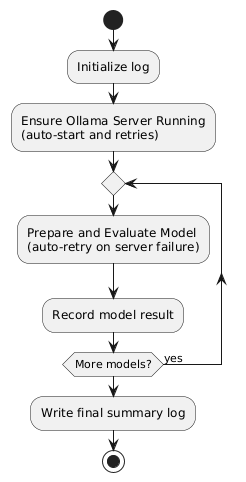
\includegraphics[width=0.6\textwidth]{figs/ch3/3.3/model-inference-pipeline.png}
    \caption{Phase 4 batch inference workflow with error handling. The process iterates through all models, checks server health, executes lm-evaluation-harness, and logs success/failure with automatic retry on server errors.}
    \label{fig:phase4_inference}
\end{figure}


%%% EXPLAIN THE OUTPUT in JSONL. Samples vs results JSON files.






% ---------------------------------------------------------
\section{Objective 4: Rubric-Based OSQ Scoring Using LLM-as-a-Judge}
\label{sec:ch3_obj4}

\subsection{Judge Model Selection and Protocol}
\label{subsec:ch3_obj4_judge_model}

Scoring open-ended responses requires deeper understanding rather than simple string matching. This research employs LLM-as-a-judge~cite, a methodology where a frontier language model evaluates responses based on rubrics and expected answers.

%%% ADD CITATIONS FOR LLM-AS--A-JUDGE- STUDIES. UPDATE GPT3.5, 4 AS CITATIONS DICTATE.
Most published alignment studies focus on GPT-3.5 and GPT-4 ( cite here ). We therefore treat GPT-4-class results as a lower bound on the judge capability of the more recent ChatGPT models used in this work, while qualitatively validating judge reliability manually on a subset of questions.

All judge models were accessed via OpenRouter with temperature=0.0 for deterministic scoring. Each model response was independently evaluated by multiple judges, enabling inter-judge agreement analysis

The judge is treated as a second measurement instrument layered on top of the evaluated model outputs. Therefore, judge prompts, output schemas, and stability checks are retained as artifacts to support traceability.

List my judge selections here. gpt-oss-120b, gpt-5-mini

% Recommended citation (add to BibTeX):
% - Zheng et al. 2023, "Judging LLM-as-a-Judge with MT-Bench and Chatbot Arena" (NeurIPS Datasets & Benchmarks / arXiv:2306.05685)


\paragraph{Judging Approaches}

I only ended up doing the rubric-based judging for now. Did not use multiple rubrics. Cite another paper that did similar here from Zotero.

\paragraph{Rubric-Based Judging}

To assess judge consistency and reduce single-model bias, multiple judge models were employed and use the grading rubric generated in Phase 2 (Section~\ref{sec:phase2}). The LLM-as-a-judge assigns:
\begin{itemize}
    \item \textbf{Full credit} (1.0): Response meets full credit criteria
    \item \textbf{Partial credit} (0.5): Response meets partial credit criteria
    \item \textbf{No credit} (0.0): Response meets no credit criteria
\end{itemize}

Prompt structure (abridged; full prompt in Appendix~\ref{app:judge_prompts}):
<< consider adding a prompt snipet here... >> 


\paragraph{Multi-Dimensional Scoring}
The judging approach employs multi-dimensional scoring adapted from Lin \& Chen (2023)~\cite{lin2023multidim}. Each response is evaluated across five dimensions on a 0--20 scale:

\begin{enumerate}
    \item \textbf{Technical Accuracy}: Correctness of facts, principles, terminology
    \item \textbf{Conceptual Understanding}: Depth of systems thinking demonstrated
    \item \textbf{Completeness}: Coverage of required answer elements
    \item \textbf{Clarity}: Communication quality and organization
    \item \textbf{Professional Relevance}: Real-world applicability
\end{enumerate}

Figure~\ref{fig:llm-as-judge-process} illustrates the judging workflow.

The dimension scores are summed to produce a total score out of 100. Figure~\ref{fig:llm-as-judge-workflow} illustrates the judging workflow.

\begin{figure}[htbp]
    \centering
    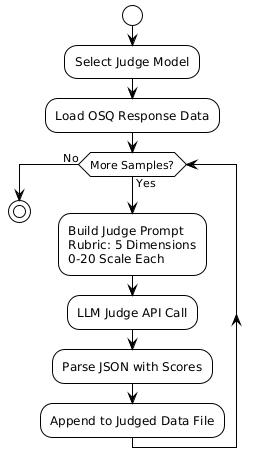
\includegraphics[width=0.4\textwidth]{figs/ch3/3.3/llm-as-judge-workflow.png}
    \caption{LLM-as-a-Judge Workflow}
    \label{fig:llm-as-judge-workflow}
\end{figure}



\subsection{Inferencing? Include the yaml reference here?}



\subsection{Judge Stability and Consistency Checks}
\label{subsec:ch3_obj4_stability}

Stability checks were performed to evaluate whether judge scores were sensitive to repeat runs under nominally identical settings. Where instability was observed, the analysis treats resulting uncertainty as part of the measurement process rather than as noise to be ignored.

%%% ADD IN INTER-JUDGE CORRELATION HERE



\subsection{(OLD, ADAPT TO NEW) OSQ-Specific Analysis}\label{sec:osq_analysis}

\subsubsection*{Analytical Question}

We characterize model performance on \acp{osq} and assess the consistency of LLM-based judges scoring responses with a multi-dimensional rubric.

\subsubsection*{Threat to Validity}

If OSQ scores are unstable or judge-specific, then model rankings and conclusions about higher-order reasoning may depend more on the choice of judge than on true model capability. This would weaken the validity of OSQ as a complementary evaluation to MCQ.

\subsubsection*{Evidence Requirements}

We require:
\begin{enumerate}[nosep]
    \item A clear description of OSQ score distributions (central tendency and variability).
    \item Evidence that different judges assign similar scores to the same models or responses.
    \item Robust estimates of mean performance that do not rely on normality assumptions.
\end{enumerate}

\subsubsection*{Visual Diagnostics}

We first inspect OSQ performance visually:
\begin{itemize}[nosep]
    \item \textbf{Score distribution plots}: for each model, histograms with kernel density estimates (KDE) show the shape, skewness, and spread of OSQ scores.
    \item \textbf{Judge-level box or violin plots}: for each judge model, we plot the distribution of assigned scores across all responses. Differences in medians or spread reveal relative leniency, strictness, or variability.
    \item \textbf{Rubric dimension bar charts}: mean scores for each rubric dimension (e.g., technical accuracy, completeness) are plotted per model, highlighting dimension-specific strengths and weaknesses.
\end{itemize}
Descriptive statistics (mean, median, standard deviation, interquartile range) are reported alongside these plots for clarity.

\subsubsection*{Statistical Tests and Assumptions}

We quantify judge consistency and uncertainty as follows:

\paragraph{Inter-judge agreement.}
For responses scored by multiple judges, we compute correlations between judges' total scores (e.g., Spearman's rank correlation). High correlation indicates that judges agree on relative performance across models or responses.

\paragraph{Bootstrap confidence intervals.}
For each model, we estimate the mean OSQ score and its uncertainty using bootstrap resampling. We draw $B$ resamples with replacement from the observed scores and compute the mean for each resample. The 2.5th and 97.5th percentiles of the bootstrap distribution form a 95\% confidence interval. This approach avoids normality assumptions and is robust to skewed or heavy-tailed score distributions.

\subsubsection*{Interpretation}

OSQ scoring reliability is  interpreted using the following decision logic:

\begin{enumerate}[nosep]
    \item \textbf{Inspect score distributions and variability.}
    \begin{itemize}[nosep]
        \item If histograms/KDE plots show roughly unimodal, well-behaved distributions with moderate spread, proceed to judge agreement.
        \item If distributions are highly skewed or multimodal, emphasize bootstrap confidence intervals and avoid parametric assumptions.
    \end{itemize}

    \item \textbf{Evaluate inter-judge agreement (correlation).}
    Let $\rho$ denote the chosen inter-judge correlation (e.g., Spearman).
    \begin{enumerate}[nosep]
        \item If $\rho \geq 0.80$: judges are strongly consistent; OSQ scores and model rankings are robust to judge choice.
        \item If $0.50 \leq \rho < 0.80$: judges show moderate agreement; OSQ results are usable but judge-specific effects should be acknowledged.
        \item If $\rho < 0.50$: judge agreement is low; treat OSQ-based conclusions with caution and highlight this as a limitation.
    \end{enumerate}

    \item \textbf{Assess uncertainty with bootstrap confidence intervals.}
    \begin{enumerate}[nosep]
        \item If bootstrap 95\% CIs for mean scores are \emph{narrow} and non-overlapping between models of interest:\\
        Mean OSQ performance differences are stable and interpretable.
        \item If CIs are \emph{wide} or heavily overlapping:\\
        Model rankings may be unreliable; report that OSQ performance differences are uncertain and may not be statistically meaningful.
    \end{enumerate}

    \item \textbf{Final interpretation.}
    \begin{itemize}[nosep]
        \item \emph{High reliability:} $\rho \geq 0.80$ and narrow CIs. OSQ results provide a trustworthy view of model performance and higher-order reasoning.
        \item \emph{Moderate reliability:} $0.50 \leq \rho < 0.80$ and/or mixed CI widths. OSQ results are informative but should be interpreted alongside MCQ results and with judge effects in mind.
        \item \emph{Low reliability:} $\rho < 0.50$ and wide CIs. OSQ results primarily illustrate trends rather than precise rankings and should be framed as exploratory.
    \end{itemize}
\end{enumerate}





\subsection{Error Handling and Adjudication Rules}
\label{subsec:ch3_obj4_error_handling}

re-running if certain errors etc, pull from chapter 5 limitations section

%%%%%
I think we should move all of this up to the environment section, since it's indempotent and did this for every section.
%%%%%



% ---------------------------------------------------------
\section{Objective 5: Robustness, Cross-Modality Evidence, and Uncertainty Quantification}
\label{sec:ch3_obj5}

\subsection{Operational Definition of MCQ Robustness}
\label{subsec:ch3_obj5_robustness}

\subsection{MCQ Position Bias Analysis (MERGE WITH ABOVE)}\label{sec:position_bias_analysis}

Position bias refers to systematic preference for particular answer positions (A, B, C, D) independent of question content. Such bias can inflate or deflate apparent model accuracy depending on the distribution of correct answers in the benchmark.

\subsubsection*{Analytical Question}

We test whether a model's multiple-choice accuracy depends on the position of the correct option (A--D), independent of question content, using the four position-rotated variants generated in \ref{sec:phase3}.

\subsubsection*{Threat to Validity}

If a model favors particular answer positions (e.g., over-selects option C), its accuracy can be artificially inflated or deflated depending on the benchmark's answer-position distribution. In that case, reported MCQ accuracy may reflect positional heuristics rather than genuine understanding, and cross-model comparisons become unfair.

\subsubsection*{Evidence Requirements}

We require evidence that:
\begin{enumerate}[nosep]
    \item Accuracy differs across positions (global position effects).
    \item Correctness for the \emph{same} questions changes across rotated variants (within-item effects).
    \item The magnitude of any position effects is quantified, not just their statistical significance.
\end{enumerate}

\subsubsection*{Visual Diagnostics}

Position bias is first assessed visually using per-position accuracy metrics. For each model, accuracy is calculated separately for each position variant:
\begin{align}
\text{Acc}_A &= \frac{\text{\# correct on variant A}}{1144} \\
\text{Acc}_B &= \frac{\text{\# correct on variant B}}{1144} \\
\text{Acc}_C &= \frac{\text{\# correct on variant C}}{1144} \\
\text{Acc}_D &= \frac{\text{\# correct on variant D}}{1144}
\end{align}

Under the null hypothesis of no position bias, $\text{Acc}_A = \text{Acc}_B = \text{Acc}_C = \text{Acc}_D$.
Deviation from the expected uniform distribution is quantified as:
\begin{equation}
\Delta_p = \text{Acc}_p - \frac{1}{4}\sum_{i \in \{A,B,C,D\}} \text{Acc}_i.
\end{equation}

We then construct the following diagnostics:
\begin{itemize}[nosep]
    \item \textbf{Accuracy-by-position bar charts}: for each model, we plot accuracy when the correct answer appears in positions A, B, C, and D. Large differences between bars indicate potential position bias.
    \item \textbf{Deviation-from-uniform plots}: for each model and position $p \in \{A,B,C,D\}$, we display $\Delta_p$ as a bar chart or heatmap. Positive values indicate preference for a position; negative values indicate avoidance.
\end{itemize}

These plots provide an immediate qualitative indication of positional preferences before formal hypothesis testing.

\subsubsection*{Statistical Tests and Assumptions}

To assess answer-position bias in MCQ evaluation, we use two complementary nonparametric hypothesis tests, each paired with a standardized effect size. Together, these tests distinguish between global position dependence and within-item position sensitivity.
We then apply the following tests:

\paragraph{Chi-square test of independence.}
For each model, we construct a $2 \times 4$ contingency table of correctness (correct/incorrect) by answer position and apply a chi-square test of independence. This tests whether correctness is independent of answer position at the aggregate level.

\paragraph{Friedman test.}
Because the four position variants share the same underlying questions, correctness across positions forms a repeated-measures design. We apply the Friedman test to test whether per-question correctness differs systematically across positions.

\paragraph{Effect size (Cramér's V).}
For the chi-square result, we compute Cramér's $V$ as
\[
    V = \sqrt{\frac{\chi^2}{N \cdot \min(r-1, c-1)}},
\]
where $N$ is the total number of observations and $r$ and $c$ are the numbers of rows and columns. This quantifies the strength of association between position and correctness.

\paragraph{KENDALLS}





\begin{itemize}[leftmargin=*, itemsep=0.5em]

\item \textbf{Chi-square test of independence} ($\chi^2$) with \textbf{Cram\'{e}r's $V$}:
  \begin{itemize}[leftmargin=*, itemsep=0.25em]
    \item \emph{Data / design:} Nominal categorical counts in a contingency table, with correctness ($\in\{\text{correct},\text{incorrect}\}$) cross-tabulated by answer position ($\in\{A,B,C,D\}$).
    \item \emph{What it tests:} Whether aggregate correctness is independent of answer position across all items.
    \item \emph{Interpretation:} A significant result indicates global position dependence, meaning some answer positions are associated with higher or lower correctness rates than expected by chance.
    \item \emph{Effect size:} Cram\'{e}r's $V$ quantifies the practical magnitude of this association, mitigating the tendency for large sample sizes to render trivial effects statistically significant.
  \end{itemize}

\item \textbf{Friedman test} (repeated measures) ($\chi^2_F$) with \textbf{Kendall's $W$}:
  \begin{itemize}[leftmargin=*, itemsep=0.25em]
    \item \emph{Data / design:} Repeated-measures design using matched items, where the same questions are evaluated across multiple rotated answer-position variants.
    \item \emph{What it tests:} Whether per-item correctness differs systematically across answer positions.
    \item \emph{Interpretation:} A significant result indicates within-item position sensitivity, meaning identical questions are more or less likely to be answered correctly depending on where the correct option appears.
    \item \emph{Effect size:} Kendall's $W$ summarizes the strength of systematic agreement across positions, with larger values indicating stronger and more consistent position effects.
  \end{itemize}

\end{itemize}


\subsubsection*{Interpretation}

The position bias results are interpreted using the following decision logic:

\begin{figure}[htbp]
    \centering
    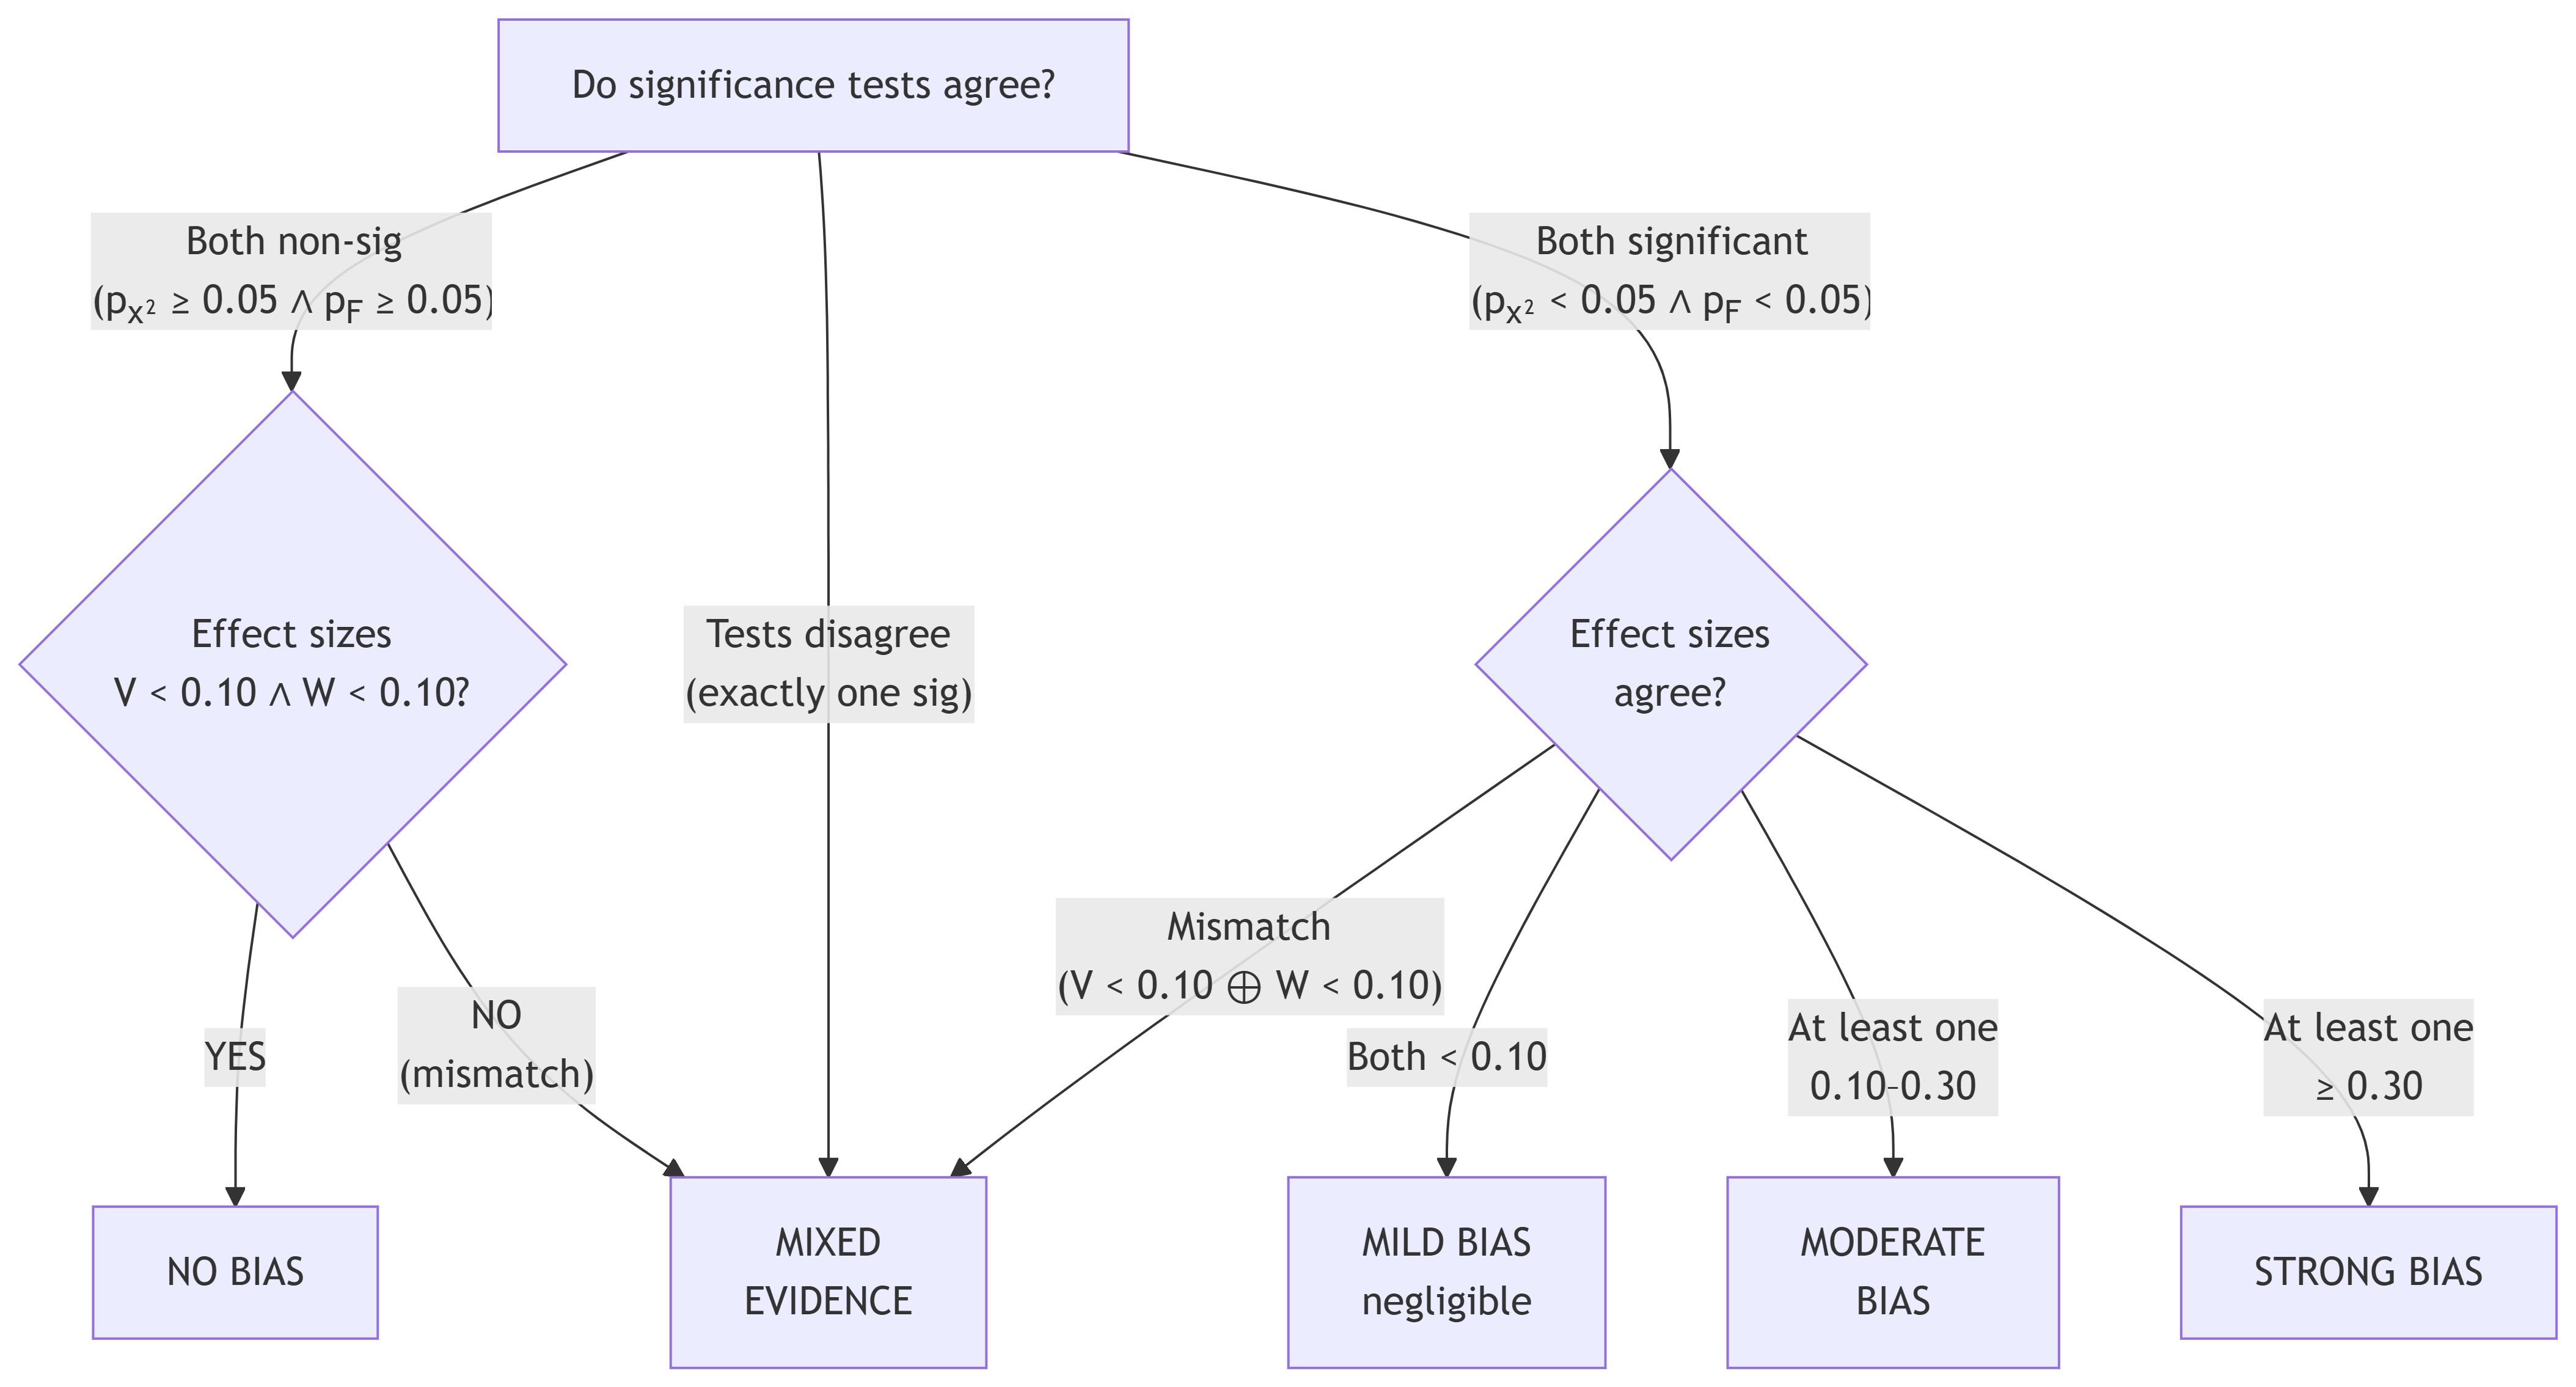
\includegraphics[width=0.9\textwidth]{figs/ch3/3.5/mcq-bias-decision-tree.png}
    \caption{MCQ Statistical Interpretation Decision Tree}
    \label{fig:mcq-statistical-interp-decision-treee}
\end{figure}

\begin{enumerate}[nosep]
    \item \textbf{Check global position dependence (chi-square).}
    \begin{enumerate}[nosep]
        \item If the chi-square test is \emph{not significant} ($p \geq 0.05$):\\
        Conclude that there is no evidence of global position bias for this model. Proceed to Step~2 to verify that any residual effects are negligible.
        \item If the chi-square test is \emph{significant} ($p < 0.05$):\\
        Conclude that correctness depends on answer position at the aggregate level. Continue with effect size and within-question analysis.
    \end{enumerate}

    \item \textbf{Assess magnitude of global bias (Cramér's $V$).}
    \begin{enumerate}[nosep]
        \item If $V < 0.10$: global position effects are negligible in practice, even if statistically significant.
        \item If $0.10 \leq V < 0.30$: position bias is moderate and should be reported as a potential source of distortion.
        \item If $V \geq 0.30$: position bias is strong and substantially affects measured accuracy; MCQ results for this model should be interpreted with caution.
    \end{enumerate}

    \item \textbf{Check within-question effects (Friedman test).}
    \begin{enumerate}[nosep]
        \item If the Friedman test is \emph{not significant} ($p \geq 0.05$):\\
        Correctness for individual questions does not change systematically across rotated positions. Any bias is mainly global and small if $V$ is small.
        \item If the Friedman test is \emph{significant} ($p < 0.05$):\\
        Per-question correctness is sensitive to position. This indicates structural position bias beyond random fluctuations and reinforces any global effects seen in Steps~1--2.
    \end{enumerate}

    %%% UPDATE BELOW FOR KENADALL'S FOR MAGNITUDE
    \item \textbf{Check within-question effects (Friedman test).}
    \begin{enumerate}[nosep]
        \item If the Friedman test is \emph{not significant} ($p \geq 0.05$):\\
        Correctness for individual questions does not change systematically across rotated positions. Any bias is mainly global and small if $V$ is small.
        \item If the Friedman test is \emph{significant} ($p < 0.05$):\\
        Per-question correctness is sensitive to position. This indicates structural position bias beyond random fluctuations and reinforces any global effects seen in Steps~1--2.
    \end{enumerate}

\end{enumerate}



We employed non-parametric inferential statistical tests to evaluate both statistical significance and effect magnitude. Specifically, the Chi-Square test of independence ($\chi^2$) was used to assess categorical associations, with Cram\'{e}r's~$V$ reported as the corresponding effect size. 
For repeated-measures analyses, the Friedman test ($Q$) was applied, and Kendall's~$W$ was reported to quantify effect magnitude.




\begin{table}[htbp]
\centering
\caption{Decision rubric for MCQ position bias classification using global and within-item evidence.}
\label{tab:position_bias_rubric}
\resizebox{\linewidth}{!}{%
\begin{tabular}{p{3.1cm} p{2.2cm} p{2.2cm} p{3.6cm} p{4.9cm}}
\toprule
\textbf{Classification} & \textbf{$p_{\chi^2}$} & \textbf{$p_{\text{Friedman}}$} & \textbf{Effect sizes} & \textbf{Interpretation / Action} \\
\midrule

No bias &
$\ge 0.05$ &
$\ge 0.05$ &
\makecell[l]{$V < 0.10$ \\ $W < 0.10$} &
No evidence that correctness depends on answer position. Report MCQ accuracy as position-invariant. \\


\addlinespace
Mixed evidence &
\multicolumn{2}{p{4.4cm}}{\makecell[l]{Tests disagree:\\
$p_{\chi^2}<0.05,\ p_{\text{Friedman}}\ge 0.05$\\
\textbf{or}\\
$p_{\text{Friedman}}<0.05,\ p_{\chi^2}\ge 0.05$}} &
\makecell[c]{(any)} &
Tests disagree (exactly one significant). Evidence is inconsistent; report diagnostics and avoid strong claims. \\

\addlinespace
Mixed evidence &
\multicolumn{2}{p{4.4cm}}{\centering (any)} &
\makecell[l]{Mismatch:\\
$V<0.10$ $\land$ $W\ge 0.10$\\
\textbf{or}\\
$V\ge 0.10$ $\land$ $W<0.10$} &
Effect sizes disagree. Evidence is inconsistent; report diagnostics and avoid strong claims. \\

\addlinespace
\makecell[l]{Mild bias \\ (negligible)} &
\multicolumn{2}{p{4.4cm}}{\makecell[l]{At least one test significant:\\
$p_{\chi^2}<0.05$\\
\textbf{or}\\
$p_{\text{Friedman}}<0.05$}} &
\makecell[l]{$V < 0.10$ \\ $W < 0.10$} &
At least one test detects a position effect, but magnitude is negligible. Report as a minor validity concern (likely sample-size sensitive); interpret primarily via effect sizes. \\

\addlinespace
Moderate bias &
$< 0.05$ &
$< 0.05$ (preferred) &
\makecell[l]{$0.10 \le V < 0.30$ \\ and/or \\ $0.10 \le W < 0.30$} &
Meaningful position dependence; accuracy comparisons may be distorted. Report and interpret MCQ results with caution. \\

\addlinespace
Strong bias &
$< 0.05$ &
$< 0.05$ &
\makecell[l]{$V \ge 0.30$ \\ and/or \\ $W \ge 0.30$} &
Position strongly confounds measured accuracy. Treat MCQ accuracy as contaminated by positional heuristics. \\

\bottomrule
\end{tabular}
}
\vspace{0.5em}
\footnotesize
\textit{Notes.} $V$ denotes Cram\'{e}r's $V$, which measures the strength of association between answer position and correctness at the aggregate (global) level.  $W$ denotes Kendall's $W$, which measures the degree of within-item agreement in correctness across answer positions (item-level position sensitivity). 
Both effect sizes quantify practical magnitude independent of sample size.

\end{table}



\subsection{Cross-Modality Comparison Framework}
\label{subsec:ch3_obj5_modality_comparison}

\subsubsection*{Analytical Question}

We test whether multiple-choice (MCQ) and open short-answer (OSQ) formats produce consistent assessments of model capability on the same underlying questions, or whether they capture different aspects of performance.

\subsubsection*{Threat to Validity}

If MCQ and OSQ results diverge, it is not valid to treat scores from the two formats as interchangeable. A model that performs well on MCQ may not perform equally well on OSQ, and overall conclusions about model capability will depend on format choice.

\subsubsection*{Evidence Requirements}

We require:
\begin{enumerate}[nosep]
    \item A measure of association between MCQ accuracy and OSQ scores across models.
    \item A paired comparison of per-model performance across formats on the matched question subset.
    \item A standardized effect size describing any systematic difference between formats.
\end{enumerate}

\subsubsection*{Visual Diagnostics}

We first compare formats visually using a scatter plot:
\begin{itemize}[nosep]
    \item \textbf{MCQ--OSQ scatter plot}: each point represents a model, with MCQ accuracy (on the matched subset) on the $x$-axis and mean OSQ score (normalized to $[0,1]$ if desired) on the $y$-axis. We overlay a least-squares regression line and a diagonal reference line $y=x$.
\end{itemize}
Points close to the diagonal indicate similar performance across formats; systematic deviations above or below the diagonal indicate models that perform better in one format than the other.

\subsubsection*{Statistical Tests and Assumptions}

We then quantify the relationship between formats:

\paragraph{Correlation between formats.}
We compute Pearson's correlation coefficient to measure linear association between MCQ accuracy and OSQ mean scores, and Spearman's rank correlation to measure agreement in model ranking. High correlation indicates that models that perform well on MCQ also tend to perform well on OSQ.

\paragraph{Paired difference test.}
For each model, we compute the difference between MCQ accuracy and normalized OSQ mean score, $\Delta_i = \text{Acc}_{\text{MCQ},i} - \bar{S}_{\text{OSQ},i}'$. We apply the Wilcoxon signed-rank test to the set of differences $\{\Delta_i\}$ to test whether the median difference is zero. This non-parametric test does not assume normally distributed differences.

\paragraph{Effect size.}
We compute Cohen's $d$ for paired samples to quantify the magnitude of the format difference:
\[
    d = \frac{\bar{\Delta}}{s_{\Delta}},
\]
where $\bar{\Delta}$ is the mean of the per-model differences and $s_{\Delta}$ is their standard deviation.

\subsubsection*{Interpretation}

The relationship between MCQ and OSQ formats is interpreted using the following decision logic:

\begin{enumerate}[nosep]
    \item \textbf{Inspect the MCQ--OSQ scatter plot.}
    \begin{itemize}[nosep]
        \item Points close to the diagonal $y=x$ suggest similar performance across formats.
        \item Systematic deviations above or below the diagonal suggest models that are relatively stronger in one format.
    \end{itemize}

    \item \textbf{Quantify association (Pearson and Spearman correlations).}
    \begin{enumerate}[nosep]
        \item If both correlations are $\geq 0.80$:\\
        MCQ and OSQ largely agree on model ordering; they measure closely related constructs.
        \item If correlations are in $[0.50, 0.80)$:\\
        Formats are moderately aligned but capture partially distinct capabilities.
        \item If either correlation is $< 0.50$:\\
        Formats diverge; MCQ and OSQ should be treated as measuring different aspects of performance.
    \end{enumerate}

    \item \textbf{Test for systematic differences (Wilcoxon signed-rank).}
    Let $\Delta_i = \text{Acc}_{\text{MCQ},i} - \bar{S}'_{\text{OSQ},i}$ be the per-model differences.
    \begin{enumerate}[nosep]
        \item If the Wilcoxon test is \emph{not significant} ($p \geq 0.05$):\\
        There is no evidence that one format systematically yields higher scores across models.
        \item If the Wilcoxon test is \emph{significant} ($p < 0.05$):\\
        One format consistently gives higher scores (direction indicated by the sign of $\bar{\Delta}$).
    \end{enumerate}

    \item \textbf{Assess practical importance (Cohen's $d$ for paired differences).}
    \begin{enumerate}[nosep]
        \item $|d| < 0.20$: negligible format difference.
        \item $0.20 \leq |d| < 0.50$: small difference; format matters somewhat.
        \item $0.50 \leq |d| < 0.80$: medium difference; format choice has clear practical impact.
        \item $|d| \geq 0.80$: large difference; MCQ and OSQ should be treated as distinct evaluations.
    \end{enumerate}

    \item \textbf{Final interpretation.}
    \begin{itemize}[nosep]
        \item \emph{Formats largely equivalent:} high correlations, non-significant Wilcoxon result, and $|d| < 0.20$.
        \item \emph{Formats partially overlapping:} moderate correlations and small-to-medium $|d|$; MCQ and OSQ both contribute complementary information.
        \item \emph{Formats clearly distinct:} low correlations and medium-to-large $|d|$; conclusions should distinguish between MCQ-style and OSQ-style capability.




% ---------------------------------------------------------
\section{Objective 6: Token-Efficiency and Cost Trade-Space Analysis}
\label{sec:ch3_obj6}

\subsection{Token Measurement Methodology}
\label{subsec:ch3_obj6_token_method}

Token usage was measured for each evaluation condition as the sum of prompt tokens and completion tokens. For OSQ evaluation, total token usage ONLY includes both model generation, not judge scoring passes. Token logs were retained per item and per run configuration to enable granular analysis of cost drivers.




\subsection{Response Length Regimes and Constraints}
\label{subsec:ch3_obj6_length_regimes}

To evaluate the quality--token trade space, response length regimes were implemented by constraining OSQ answers to a maximum of 500 tokens.

\subsection{Cost Modeling Assumptions}
\label{subsec:ch3_obj6_cost_model}

%%% IF I END UP ACTUALLY DOING A COST PER INFERENCE SECTION. i THINK WE SHOULD STAY AWAY FROM THIS FOR NOW AND STAY FOCUSED ON THE AMOUNT OF TOKENS, WHICH IS TEMPORALLY AGNOSTIC
Costs were computed by mapping token usage to published per-token pricing for API-accessed models and to compute proxies for local inference where appropriate. Because pricing schedules can change over time and differ across providers, the dissertation reports token counts as the primary stable quantity and treats cost estimates as contextualized calculations rather than immutable facts.


\subsection{Quality--Token Trade-Space Analysis}
\label{subsec:ch3_obj6_trade_space}



\subsection{Tokenomics and Cost-Effectiveness Analysis (MERGE WITH ABOVE}\label{sec:tokenomics}

%%% CONSIDER ADDING THIS PARAGRAPH HERE TO TIE CH3 BACK TO CH2.
% \paragraph{What this dissertation reports and why (link to RQ3).}
% Consistent with treating cost as a trade-space variable rather than a qualification criterion, this dissertation reports compute-relevant quantities to contextualize evaluation feasibility and to enable replication and comparison. In particular, the study tracks (i) token counts associated with prompts and responses, (ii) how response length policies (e.g., short vs.\ long outputs) change total token consumption, and (iii) when OSQ scoring involves judge-based evaluation, the additional call structure and token overhead implied by the judge pipeline. These quantities support the dissertation's analysis of modality- and length-dependent computational cost and token efficiency (RQ3) without asserting that lower cost implies higher qualification. Instead, cost-aware reporting clarifies the feasible evidence envelope under which robustness checks, replications, and OSQ scoring can be conducted, and it motivates evaluation designs that are transparent about the computational resources required to produce a given level of evidence.



\subsubsection*{Analytical Question}

We evaluate how models trade off quality and cost by quantifying token usage, monetary cost, and efficiency, and by identifying models that are Pareto-optimal in terms of cost-effectiveness.

\subsubsection*{Threat to Validity}

Reporting accuracy or OSQ scores alone may favor models that are prohibitively expensive to deploy at scale. Without incorporating cost, conclusions about ``best'' models may be impractical for real-world use, especially in large-scale evaluation or operational settings.

\subsubsection*{Evidence Requirements}

We require:
\begin{enumerate}[nosep]
    \item Token counts per response (prompt and completion) for each model.
    \item Per-model cost estimates based on provider pricing.
    \item At least one scalar efficiency metric linking cost or tokens to quality.
    \item A way to identify models that are not dominated by cheaper or better alternatives.
\end{enumerate}

\subsubsection*{Visual Diagnostics}

We summarize cost–quality trade-offs visually:
\begin{itemize}[nosep]
    \item \textbf{Pareto frontier plot}: models are plotted with cost per response (or per 1{,}000 questions) on the $x$-axis and mean OSQ quality on the $y$-axis. Models on the upper-left boundary form the Pareto frontier.
    \item \textbf{Cost-quality chart}: a bubble or bar chart shows cost per 1{,}000 evaluated questions alongside mean OSQ score, making high-cost versus high-value models easy to distinguish.
\end{itemize}

\subsubsection*{Cost and Efficiency Metrics}

For each model, we compute token and cost statistics:
\begin{itemize}[nosep]
    \item \textbf{Token counts}: average prompt tokens $T_{\text{input}}$, completion tokens $T_{\text{output}}$, and total tokens $T_{\text{total}} = T_{\text{input}} + T_{\text{output}}$ per OSQ response.
    \item \textbf{Monetary cost}: given input and output prices $P_{\text{input}}$ and $P_{\text{output}}$ (USD per million tokens), the expected cost per response is
    \[
        \text{Cost}_{\text{response}} = T_{\text{input}} \cdot \frac{P_{\text{input}}}{10^6} + T_{\text{output}} \cdot \frac{P_{\text{output}}}{10^6}.
    \]
    This can be scaled to cost per 1{,}000 questions.
    \item \textbf{Efficiency metric}: we report a single scalar metric such as cost per score point,
    \[
        \text{Cost-per-score} = \frac{\text{Cost}_{\text{response}}}{\bar{S}_{\text{OSQ}}},
    \]
    where $\bar{S}_{\text{OSQ}}$ is the mean OSQ score. Lower values indicate better cost-effectiveness.
\end{itemize}

% \begin{itemize}
%     \item \textbf{Cost vs. Accuracy scatter}: Models plotted by cost/sample (x-axis) and accuracy (y-axis)
%     \item \textbf{Efficiency frontier}: Convex hull of models representing Pareto-optimal cost-accuracy tradeoffs
%     \item \textbf{ROI curves}: ROI as function of benchmark scale for different model pairs
%     \item \textbf{Token distribution histograms}: Distribution of tokens/sample for thinking vs. standard models
%     \item \textbf{Break-even plots}: Break-even point visualized as intersection of cost curves
% \end{itemize}


\subsubsection*{Interpretation}

% Models on the Pareto frontier achieve the best available trade-offs between cost and quality: no other model is both cheaper and more accurate. Models inside the frontier are dominated by at least one alternative that is strictly better in cost, quality, or both. The efficiency metric (e.g., cost per score point) provides a simple rank ordering of models by cost-effectiveness and enables practical recommendations such as ``cheaper models that achieve near-top performance'' versus ``premium models whose quality gains justify their cost.'' This analysis grounds benchmark results in realistic resource constraints.


Cost-effectiveness and token usage are  interpreted using the following decision logic:

\begin{enumerate}[nosep]
    \item \textbf{Examine the Pareto frontier plot.}
    \begin{enumerate}[nosep]
        \item Identify models on the upper-left boundary (high quality, low cost): these form the Pareto frontier.
        \item Models that lie strictly below and to the right of the frontier are dominated by at least one alternative and are less attractive.
    \end{enumerate}

    \item \textbf{Compare cost per 1{,}000 questions.}
    \begin{itemize}[nosep]
        \item If two models have similar quality but one has substantially lower cost, the cheaper model is preferred for large-scale deployment.
        \item If a more expensive model has noticeably higher quality, the trade-off depends on available budget and required performance.
    \end{itemize}

    \item \textbf{Evaluate the efficiency metric (e.g., cost-per-score).}
    \begin{enumerate}[nosep]
        \item Rank models by cost-per-score; lower values indicate better efficiency.
        \item Check whether highly efficient models also meet minimum quality thresholds (e.g., a target mean OSQ score).
    \end{enumerate}

    \item \textbf{Final interpretation.}
    \begin{itemize}[nosep]
        \item \emph{Operationally optimal models:} models on the Pareto frontier with low cost-per-score and acceptable quality; these are primary candidates for deployment.
        \item \emph{Premium models:} models with the highest quality but also much higher cost; preferable only when maximal performance is required and budget allows.
        \item \emph{Dominated models:} models that are simultaneously more expensive and less accurate than at least one alternative; these can be deprioritized.
    \end{itemize}
\end{enumerate}
    



% ---------------------------------------------------------
\section{Chapter Summary}
\label{sec:ch3_summary}

This chapter defined an objective-centered methodology for producing modality-aware, robustness-aware, and cost-aware evaluation evidence. It described the shared execution environment and reproducibility controls, then specified the procedures used to (i) curate and derive benchmark artifacts, (ii) generate OSQ grading scaffolds, (iii) execute standardized inference across MCQ and OSQ, (iv) score OSQ outputs via rubric-based judging, (v) quantify robustness and cross-modality evidence patterns under uncertainty, and (vi) evaluate token-efficiency tradeoffs into qualification guidance.


%%%%
ADD A BLURB IN HERE HOW ALL OBJECTIVES ARE ADDRESSED, EXCEPT #7! THAT WILL BE ADDRESS IN CHAPTER 5 AS A WHOLE (SYNTHESIZE QUALIFICATION GUIDANCE), IN PARTICULAR, THE GUIDANCE TABLE.
%%%%


%%% integrate below with above.
The following chapters present results (Chapter~\ref{ch:results}), discuss implications (Chapter~\ref{ch:discussion}), and conclude with recommendations for practice and future research (Chapter~\ref{ch:conclusion}).




%%%% CONSIDER INCLUSION. TAXONOMY CAN BE INFERRED FROM THE DOCUMENT STRUCTURE, MAY BE UNNECESSARY.
%  This section describes the metrics, statistical tests, and visualization approaches for each analysis dimension. A taxonomy of the analyses performed are in Figure \ref{fig:analysis-taxonomy}.

% \begin{figure}[htbp]
%     \centering
%     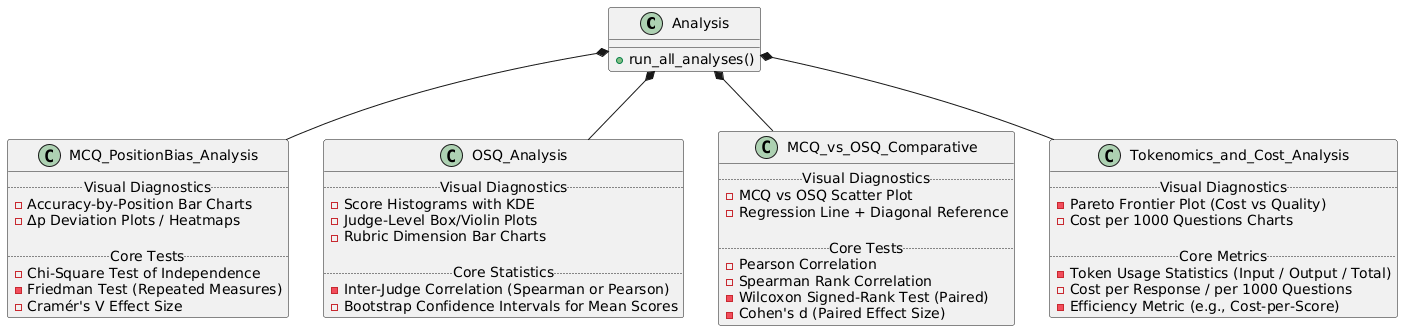
\includegraphics[width=1\textwidth]{figs/ch3/3.5/analysis-taxonomy.png}
%     \caption{Analysis Taxonomy}
%     \label{fig:analysis-taxonomy}
% \end{figure}


\clearpage










